\subsection*{Иродов 2.166}

\setcounter{equation}{0}

\begin{abstract}
Два длинных параллельных провода находятся в слабо проводящей среде с удельным сопротивлением $\rho$. Расстояние между осями проводов $\ell$, радиус сечения каждого провода $a$. Найти для случая $a << \ell$:
а) плотность тока в точке, равноудаленной от осей проводов на расстояние $r$, если разность потенциалов между проводами равна $U$;
б) сопротивление среды на единицу длины проводов.
\end{abstract}

\noindent \hrulefill
\\
\begin{wrapfigure}[6]{r}{0.30\textwidth}
	\raisebox{0pt}[\dimexpr\height-2\baselineskip\relax]{
	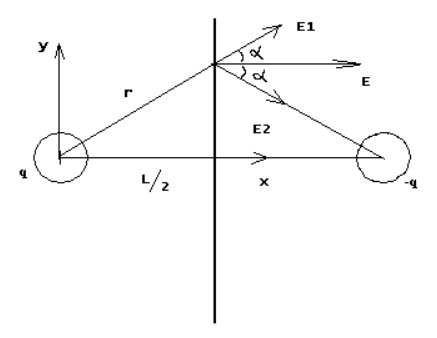
\includegraphics[width=0.30\textwidth]{pics/2.166.png}}
\end{wrapfigure}

a) $\tau$ - линейная плотность заряда провода. Согласно теореме Гаусса находим напряженность электрического поля одного провода:

$$\Phi_{E} = E. 2 \pi r . \ell,$$
$$\Phi_{E} = \frac{q}{\epsilon_0}$$

$$\xrightarrow{} E = \frac{q}{2 \pi \epsilon_0 r . l} = \frac{\tau}{2 \pi \epsilon_0 r}$$

Напряженность электрического поля на оси Ох:

$$E = E_1 + E_2 = \frac{\tau}{2 \pi \epsilon_0 x} + \frac{\tau}{2 \pi \epsilon_0 (\ell -x)}$$

Разность потенциалов между проводами:

$$U = \displaystyle \int_{a}^{\ell -a } E.dx = \frac{\tau}{2 \pi \epsilon_0}(\ln{\frac{\ell -a}{a} }- \ln{\frac{a}{\ell -a}}) = \frac{\tau}{2 \pi \epsilon_0}2\ln{\frac{\ell -a}{a} } $$

$$\xrightarrow{l \gg a} \tau = \frac{U \pi \epsilon_0}{\ln{\frac{\ell}{a}}} \quad (1)$$

Напряженность электрического поля на оси, которая равноудаленна от осей проводов на расстояние $r$: 

$$E = 2E_1 \cos{\alpha} = 2 \frac{\tau}{2 \pi \epsilon_0 r} \frac{\ell /2}{r} = \frac{\tau \ell}{2 \pi \epsilon_0 r} \quad (2)$$

Поставим (1) в (2):

$$E(r) = \frac{U \ell}{2 \ln{\frac{\ell}{a}}r^2}$$

Плотность тока:
$$j(r) = \frac{1}{\rho}.E(r) = \frac{U \ell }{2 \rho \ln{\frac{\ell}{a}r^2}}$$

б) Полный электрический ток на отрезке длиной h:

$$I = \displaystyle \int_{-\infty}^{\infty} j(r).h.dy = \frac{U \ell}{2 \rho \ln{\frac{\ell}{a}}} \times \displaystyle \int_{-\infty}^{\infty} \frac{h.dy}{(\sqrt{((\frac{\ell}{2})^2 + y^2)})^2} $$

$$I = \frac{U \ell h}{\rho \ln{\frac{\ell}{a}}} \times  \displaystyle \int_{-\infty}^{\infty} \frac{dy}{\frac{\ell^2}{4} + y^2}=  \frac{U \ell h}{\rho \ln{\frac{\ell}{a}}} \times \frac{1}{\ell/2} . arctg(\frac{y}{\ell/2}) |_{0}^{\infty} =  \frac{U \ell h}{\rho \ln{\frac{\ell}{a}}} \times \frac{1}{\ell/2} . (\frac{\pi}{2} - 0)$$

$$I = \frac{U\pi h}{\rho \ln{\frac{\ell}{a}}}$$

Удельное сопротивление:

$$R_1 = \frac{U}{I_1} = \frac{U.h}{I}  = \frac{\rho \ln{\frac{\ell}{a}}}{\pi}$$

\textbf{Ответ:}

$$a) j(r) = \frac{U \ell }{2 \rho \ln{\frac{\ell}{a}r^2}}$$

$$b) R_1 = \frac{\rho \ln{\frac{\ell}{a}}}{\pi}$$









